\chapter{Quantum Dot Results}

\section{One Dimension}
\label{app:1d_qd}

\subsection*{Four electrons}

\begin{figure}[h]
    \centering
    \makebox[\textwidth][c]{
    \begin{minipage}{0.6\textwidth}
        \centering
        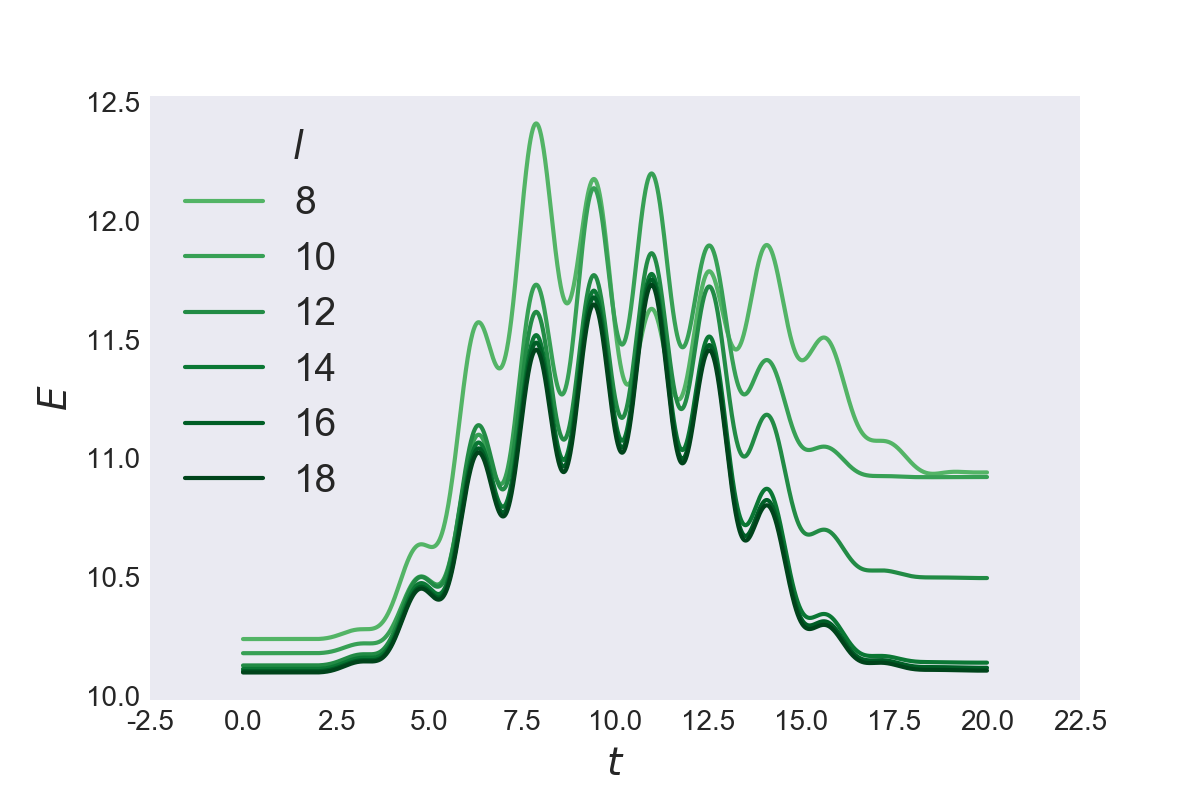
\includegraphics[width=\textwidth]{results/figures/1D/n=4energy.png}
    \end{minipage}\hfill 
    \begin{minipage}{0.6\textwidth}
        \centering 
        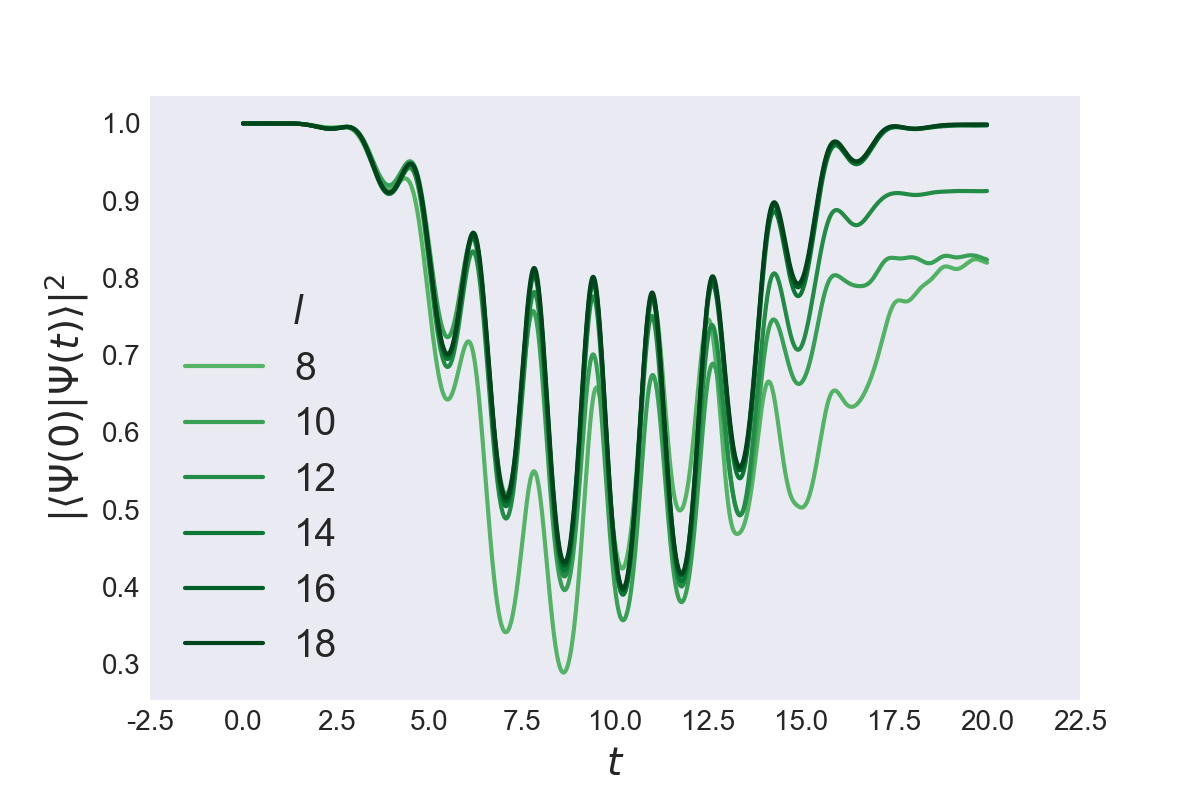
\includegraphics[width=\textwidth]{results/figures/1D/n=4overlap.png}
    \end{minipage}
    }
    \caption{Time-dependent energy (left) and ground state probability (right)
        of a one-dimensional harmonic oscillator with $\Omega=1$
        and $n=4$ electrons under the influence of a oscillating electric field 
        of frequency $\omega = 2 \Omega = 2$ and field strength $\vb{E}_\text{max}=1$,
        for different number of spin-orbitals $l=\{8,10,12,14,16,18\}$.
    }
    \label{fig:1d_n4_qd}
\end{figure}

\pagebreak

\subsection*{Six electrons}

\begin{figure}[h!]
    \centering
    \makebox[\textwidth][c]{
    \begin{minipage}{0.6\textwidth}
        \centering
        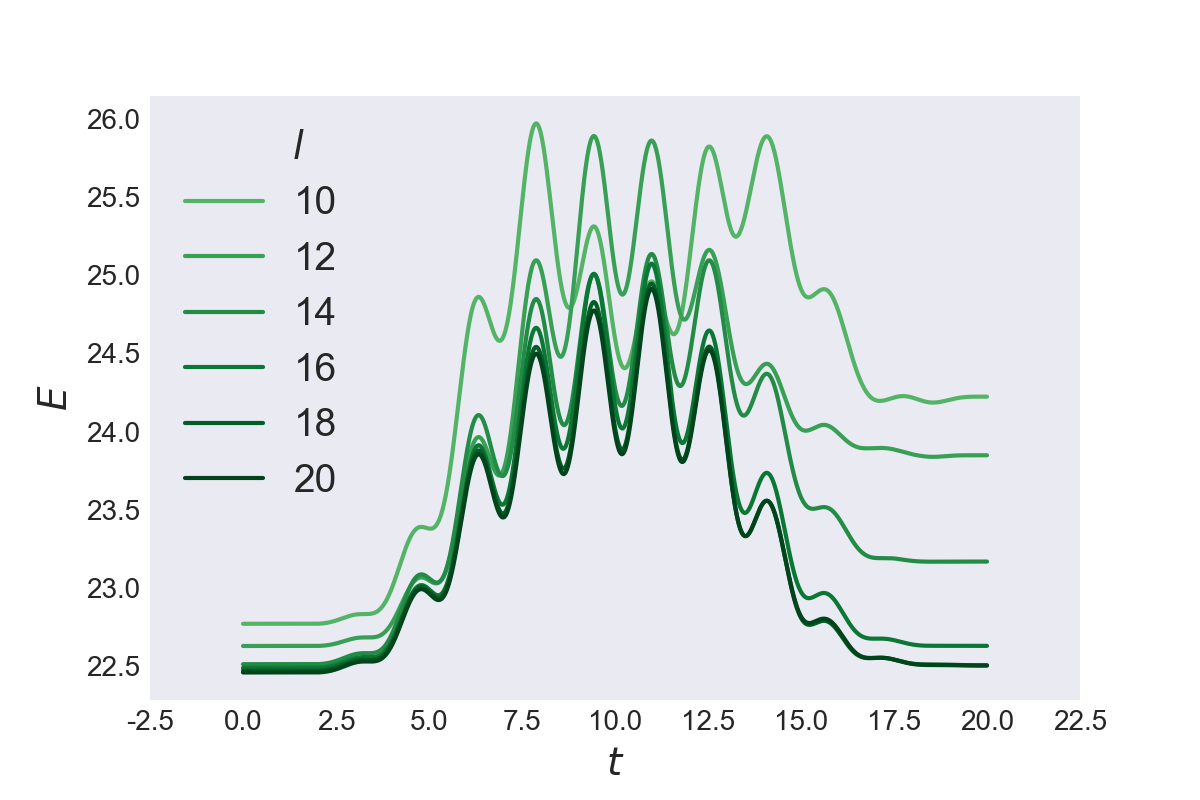
\includegraphics[width=\textwidth]{results/figures/1D/n=6energy.png}
    \end{minipage}\hfill 
    \begin{minipage}{0.6\textwidth}
        \centering 
        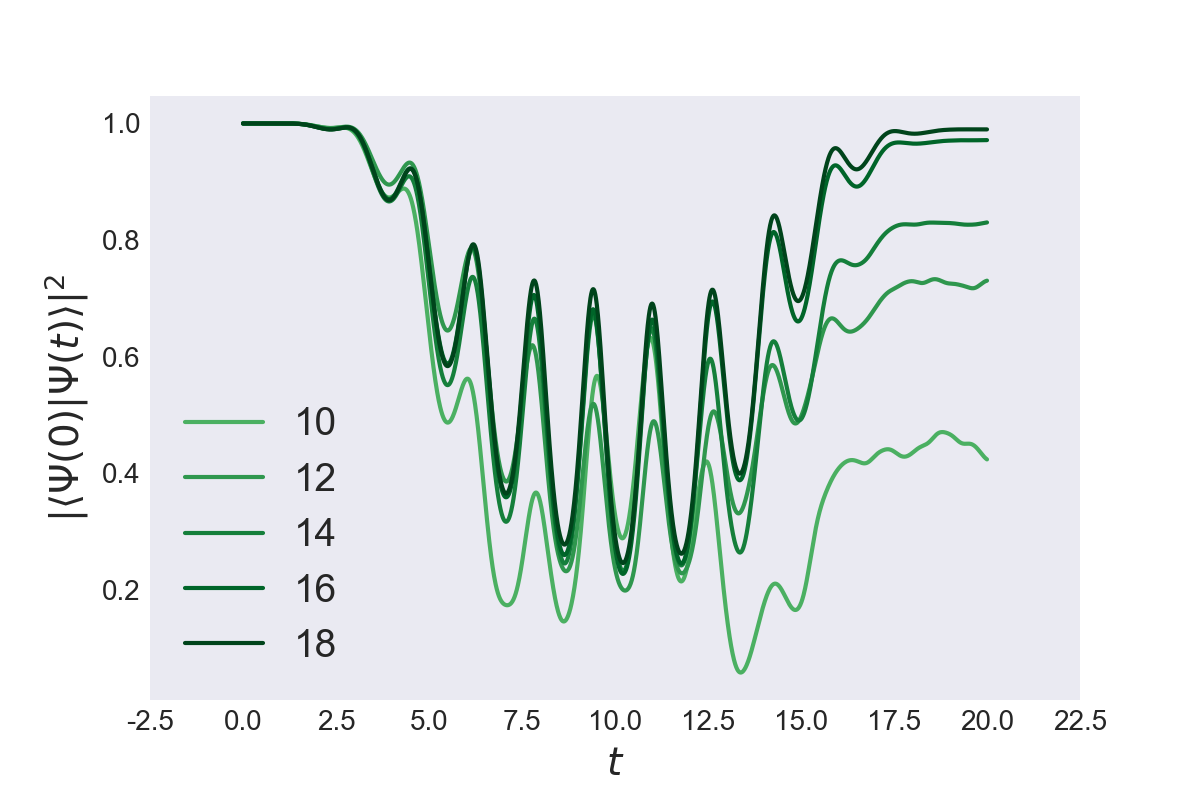
\includegraphics[width=\textwidth]{results/figures/1D/n=6overlap.png}
    \end{minipage}
    }
    \caption{Time-dependent energy (left) and ground state probability (right)
        of a one-dimensional harmonic oscillator with $\Omega=1$
        and $n=6$ electrons under the influence of a oscillating electric field 
        of frequency $\omega = 2 \Omega = 2$ and field strength $E_\text{max}=1$,
        for different number of spin-orbitals $l=\{10,12,14,16,18,20\}$.
    }
    \label{fig:1d_n6_qd}
\end{figure}

\subsection*{Eight electrons}

\begin{figure}[!h]
    \centering
    \makebox[\textwidth][c]{
    \begin{minipage}{0.6\textwidth}
        \centering
        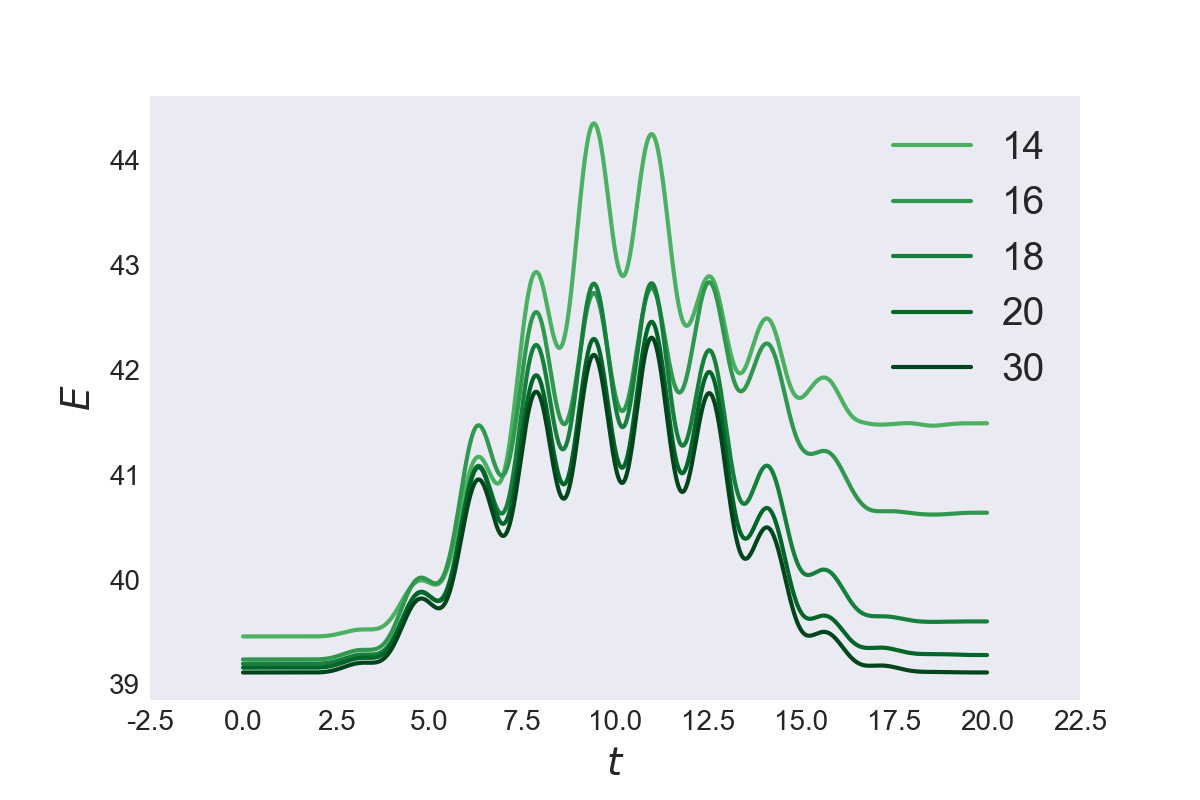
\includegraphics[width=\textwidth]{results/figures/1D/n=8energy.png}
    \end{minipage}\hfill 
    \begin{minipage}{0.6\textwidth}
        \centering 
        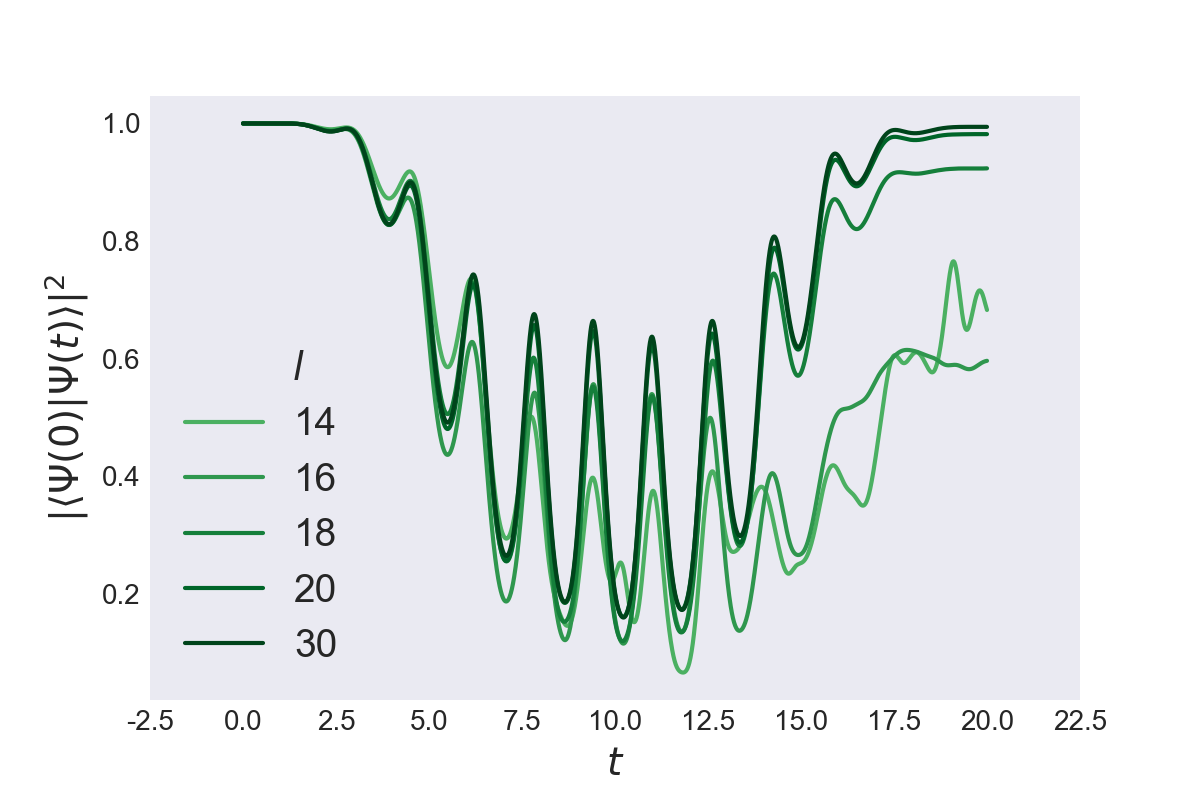
\includegraphics[width=\textwidth]{results/figures/1D/n=8overlap.png}
    \end{minipage}
    }
    \caption{Time-dependent energy (left) and ground state probability (right)
        of a one-dimensional harmonic oscillator with $\Omega=1$
        and $n=8$ electrons under the influence of a oscillating electric field 
        of frequency $\omega = 2 \Omega = 2$ and field strength $E_\text{max}=1$,
        for different number of spin-orbitals $l=\{14,16,18,20,30\}$.
    }
    \label{fig:1d_n8_qd}
\end{figure}

\pagebreak

\subsection*{Ten electrons}

\begin{figure}[!h]
    \centering
    \makebox[\textwidth][c]{
    \begin{minipage}{0.6\textwidth}
        \centering
        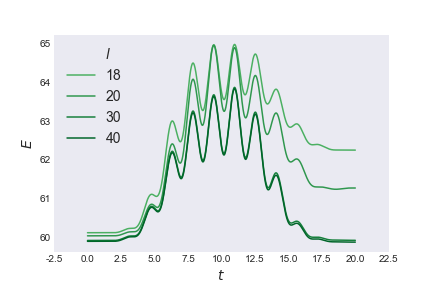
\includegraphics[width=\textwidth]{results/figures/1D/n=10energy.png}
    \end{minipage}\hfill 
    \begin{minipage}{0.6\textwidth}
        \centering 
        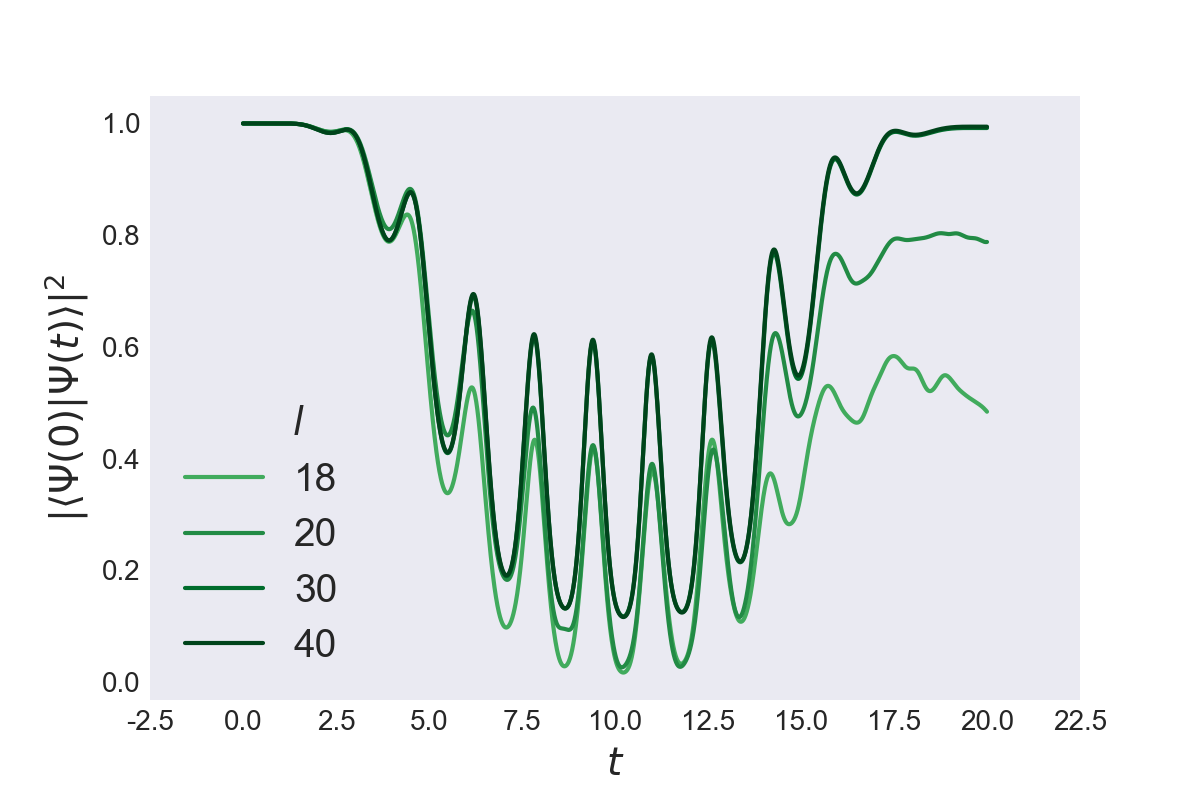
\includegraphics[width=\textwidth]{results/figures/1D/n=10overlap.png}
    \end{minipage}
    }
    \caption{Time-dependent energy (left) and ground state probability (right)
        of a one-dimensional harmonic oscillator with $\Omega=1$
        and $n=10$ electrons under the influence of a oscillating electric field 
        of frequency $\omega = 2 \Omega = 2$ and field strength $E_\text{max}=1$,
        for different number of spin-orbitals $l=\{18,20,30,40\}$.
    }
    \label{fig:1d_n10_qd}
\end{figure}

\subsection*{Twelve electrons}

\begin{figure}[!h]
    \centering
    \makebox[\textwidth][c]{
    \begin{minipage}{0.6\textwidth}
        \centering
        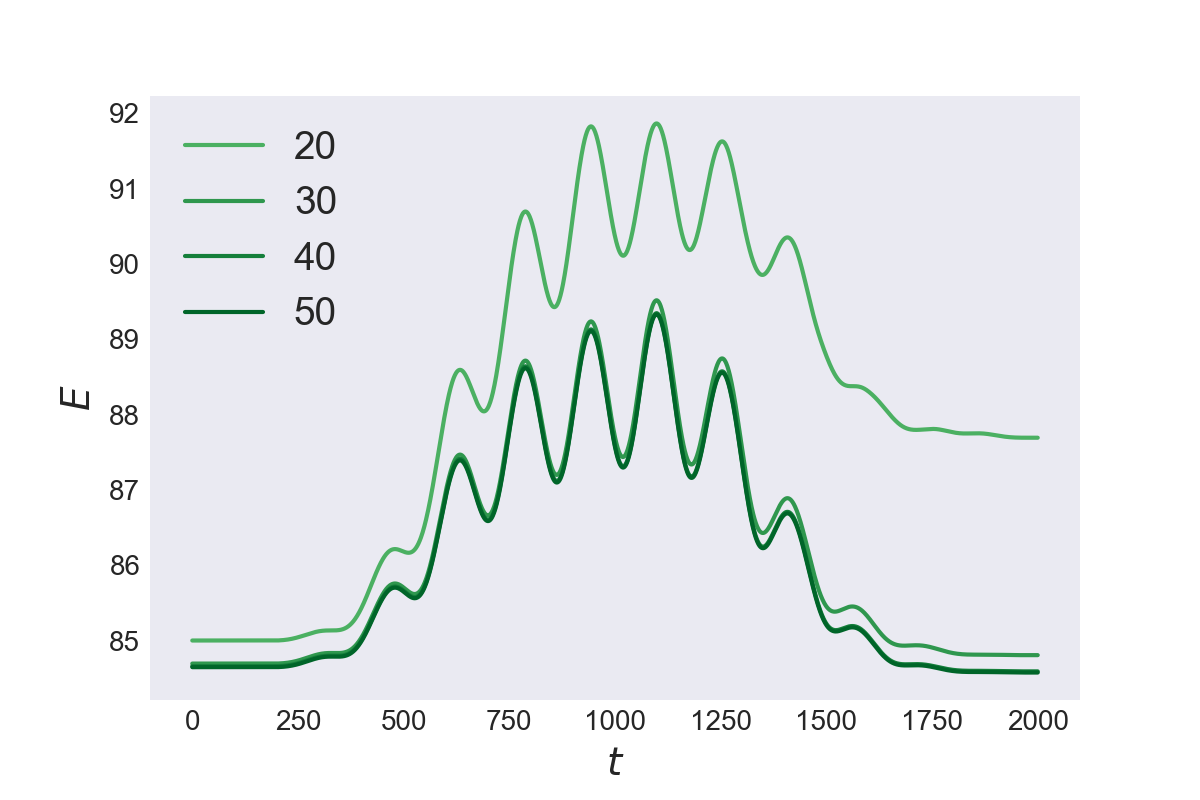
\includegraphics[width=\textwidth]{results/figures/1D/n=12energy.png}
    \end{minipage}\hfill 
    \begin{minipage}{0.6\textwidth}
        \centering 
        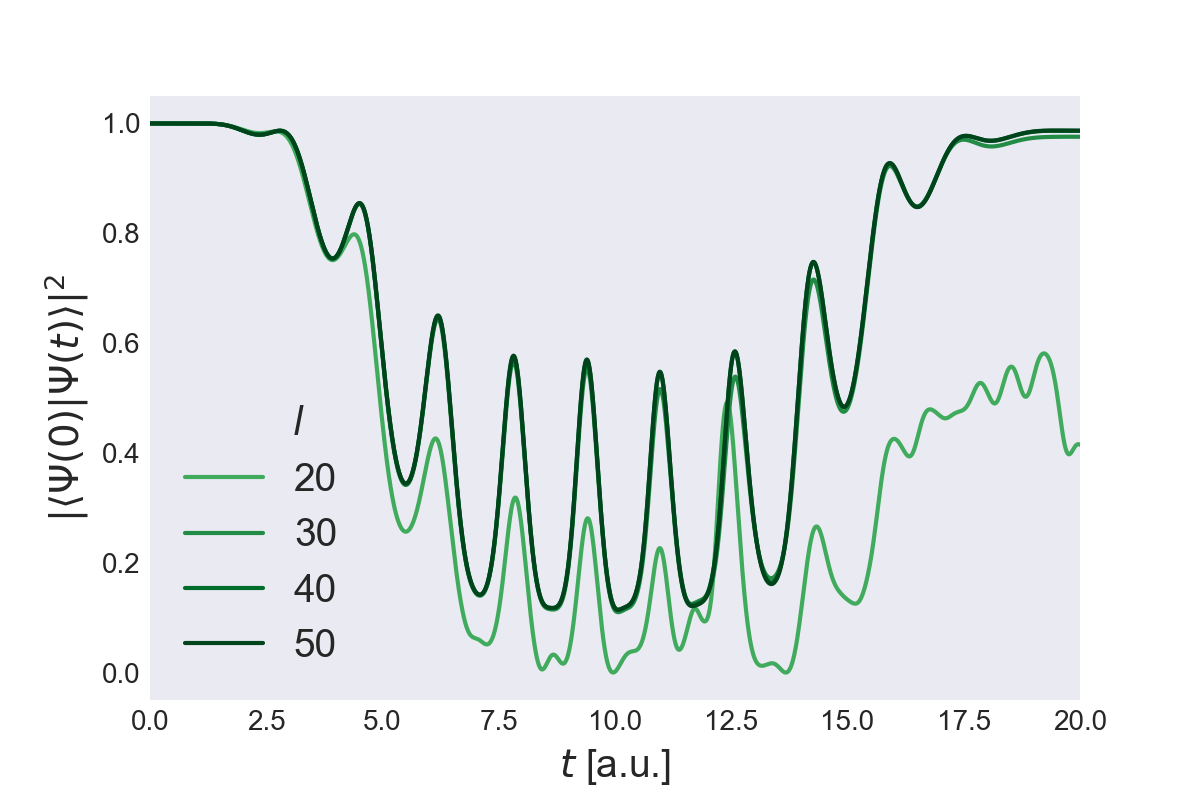
\includegraphics[width=\textwidth]{results/figures/1D/n=12overlap.png}
    \end{minipage}
    }
    \caption{Time-dependent energy (left) and ground state probability (right)
        of a one-dimensional harmonic oscillator with $\Omega=1$
        and $n=12$ electrons under the influence of a oscillating electric field 
        of frequency $\omega = 2 \Omega = 2$ and field strength $E_\text{max}=1$,
        for different number of spin-orbitals $l=\{20,30,40,50\}$.
    }
    \label{fig:1d_n12_qd}
\end{figure}

\pagebreak

\section{Two Dimensions}
\label{app:supp_2d_qd_results}

\subsection*{Two electrons}

\begin{figure}[!h]
    \centering
    \makebox[\textwidth][c]{
    \begin{minipage}{0.6\textwidth}
        \centering
        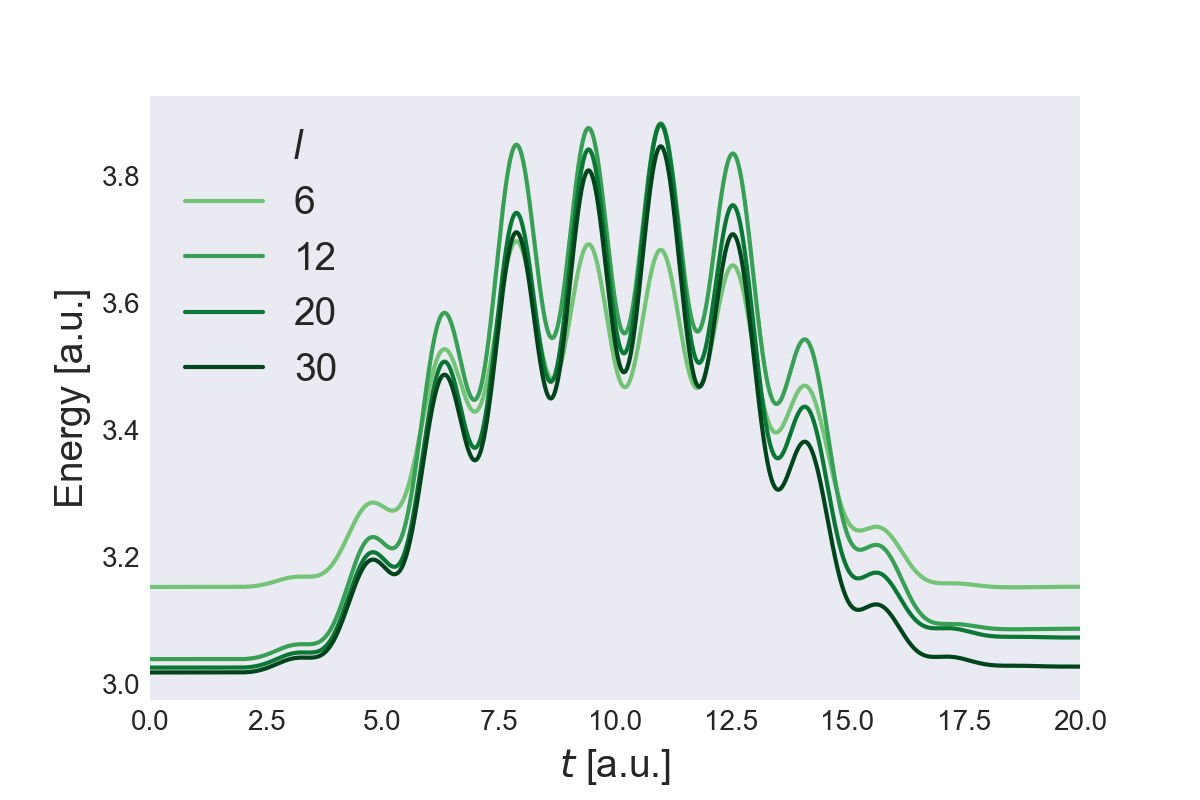
\includegraphics[width=\textwidth]{results/figures/2D/n2_energy.png}
    \end{minipage}\hfill 
    \begin{minipage}{0.6\textwidth}
        \centering 
        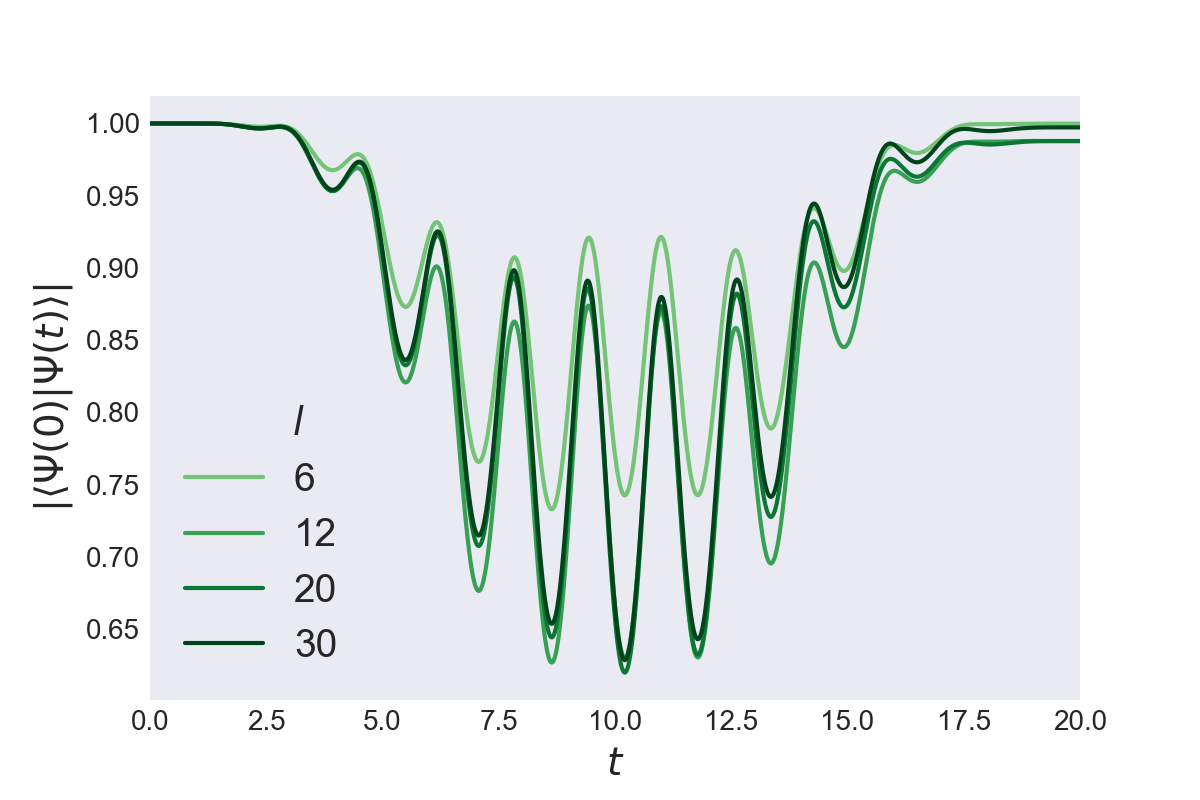
\includegraphics[width=\textwidth]{results/figures/2D/n2_overlap.png}
    \end{minipage}
    }
    \caption{Time-dependent energy (left) and ground state probability (right)
        of a two-dimensional harmonic oscillator with $\Omega=1$
        and $n=2$ electrons under the influence of a oscillating electric field 
        of frequency $\omega = 2 \Omega = 2$ and field strength $E_\text{max}=1$,
        for different number of spin-orbitals $l=\{6,12,20,30\}$.
    }
    \label{fig:2d_n2_qd}
\end{figure}


\subsection*{Six electrons}

\begin{figure}[!h]
    \centering
    \makebox[\textwidth][c]{
    \begin{minipage}{0.6\textwidth}
        \centering
        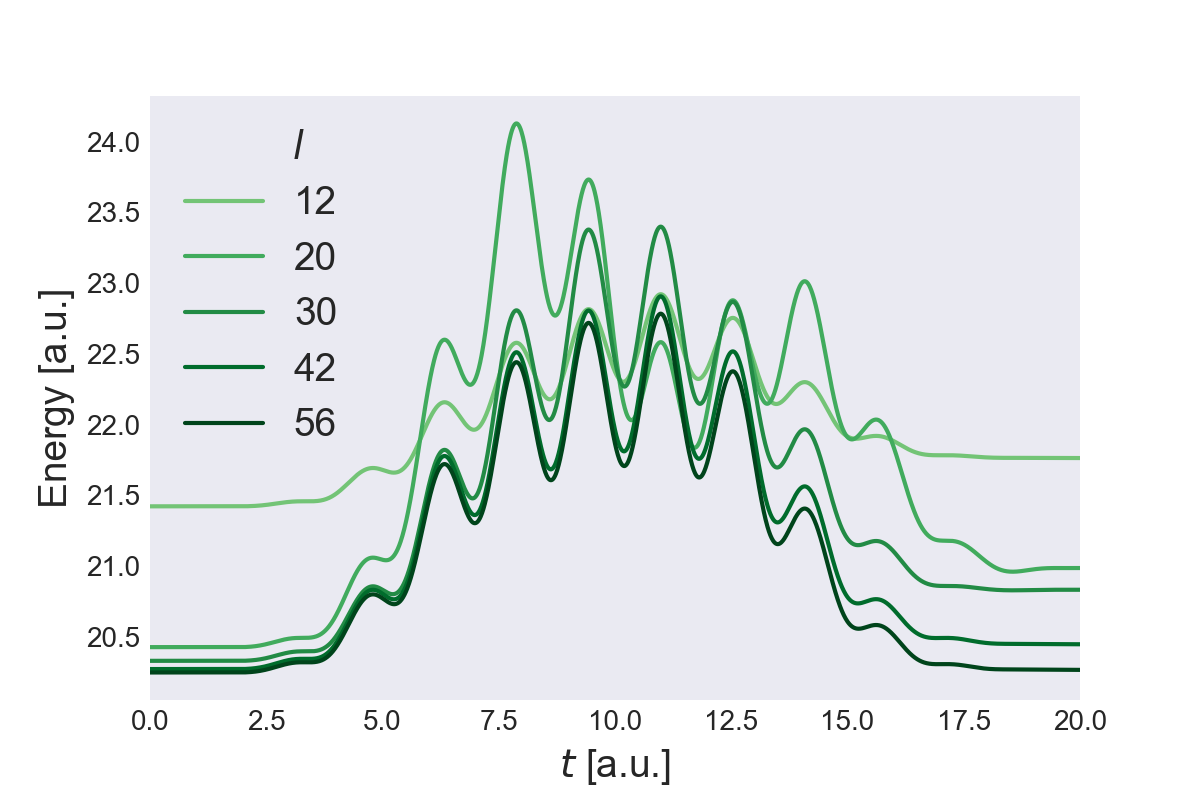
\includegraphics[width=\textwidth]{results/figures/2D/n6_energy.png}
    \end{minipage}\hfill 
    \begin{minipage}{0.6\textwidth}
        \centering 
        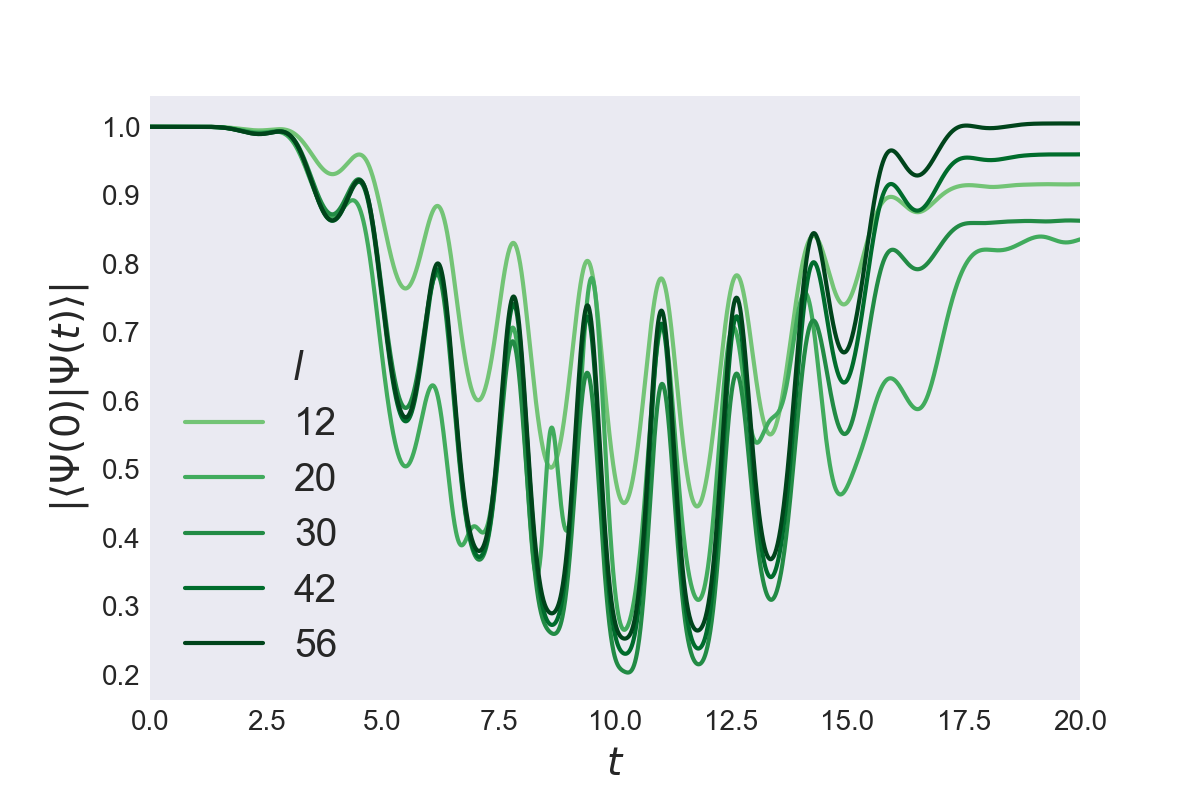
\includegraphics[width=\textwidth]{results/figures/2D/n6_overlap.png}
    \end{minipage}
    }
    \caption{Time-dependent energy (left) and ground state probability (right)
        of a two-dimensional harmonic oscillator with $\Omega=1$
        and $n=6$ electrons under the influence of a oscillating electric field 
        of frequency $\omega = 2 \Omega = 2$ and field strength $E_\text{max}=1$,
        for different number of spin-orbitals $l=\{6,12,20,30\}$.
    }
    \label{fig:2d_n6_qd}
\end{figure}
